\documentclass[10pt,aspectratio=169]{beamer}

\usetheme[progressbar=foot]{metropolis}
\usepackage{appendixnumberbeamer}

\usepackage{booktabs}
\usepackage[scale=2]{ccicons}

\usepackage{pgfplots}
\usepgfplotslibrary{dateplot}

\usepackage{xspace}
\newcommand{\themename}{\textbf{\textsc{metropolis}}\xspace}

\usepackage{tikz}

\usepackage{wrapfig}

\usepackage{appendixnumberbeamer}

\usepackage{selinput}
\usepackage{ulem}

\usepackage{tabularx}
\usepackage{subcaption}

\usepackage[final]{pdfpages}

\usepackage{amsmath}
%\usepackage[mathrm=sym]{unicode-math}
%\setmathfont{Fira Math}
%\usepackage{arevmath}


\title{Variational Autoencoders}
\subtitle{Learning generative models with latent representations}
\date{May 19, 2020}
\author{Claas Völcker}
\institute{Deep Generative Models - SoSe 2020}
% \titlegraphic{\hfill\includegraphics[height=1.5cm]{logo.pdf}}

\begin{document}
%\setlength{\metropolis@progressinheadfoot@linewidth}{100pt}

\maketitle


\begin{frame}{Table of contents}
\setbeamertemplate{section in toc}[sections numbered]
\tableofcontents[hideallsubsections]
\end{frame}


\section{Inference through optimization}

\begin{frame}{What if we replaced an inference question with optimization?}
    \begin{itemize}[<+->]
        \item The target: $$P(X)$$
        \item The hope: there is a nice $$z,~\text{so that}~P(x) = \int P(z)P(x|z)dz$$ which governs x (latent variable)
        \item I.e. all dogs look similar, if I know something is a dog, certain attributes (tails, legs, snout) are likely
        \item Idea: rephrase inference as optimization
    \end{itemize}
\end{frame}

%\begin{frame}{But we know nothing about it!}
%    \begin{itemize}
%        \item How does knowing about z help us?
%    \end{itemize}
%    \begin{align*}
%        \max_\phi \sum_x p(\phi, x)\\
%        = \max_\phi \sum_x \log p(\phi, x)\\
%        = \max_\phi \sum_x \log \int p(z) p_\phi(x | z) dz
%    \end{align*}
%    \begin{align*}
%        \sum_x \int \log \frac{p_\phi(z | x) \cdot p_\phi(x)}{p_\phi(z)}
%    \end{align*}
%\end{frame}

\begin{frame}{Working through the math - 1}

    \begin{align*}
        \onslide<+->{\text{Maximize: }P(x) \sim \int p_\phi(x|z)p_\phi(z)dz}
    \end{align*}
    \begin{itemize}[<+->]
        \item A latent variable model
        \item Assumption: there is some (hopefully small) z which governs data
        \item Define $P(z)$ and $P(x|z)$
        \item Main problem: We don't have that information for our dog
        \item Can we just ignore that problem? :D
    \end{itemize}
    \begin{align*}
        \onslide<+->{P(x|z) = \mathcal{N}(x|f(z;\phi),\sigma^2 \cdot I)}
    \end{align*}

    \begin{itemize}[<+->]
        \item $f$ is deterministic, $\mathcal{N}$ enables optimization
    \end{itemize}
\end{frame}

\begin{frame}{Working through the math - 2}
    \begin{itemize}[<+->]
        \item We could maximize by sampling? (akin to MCMC)
        \item No, too many samples would be needed
        \item Don't know if a sampled z is actually ''meant to'' produce a given x
        \item It would be great to have $P(z|x)$ for that
        \item That's just our problem in reverse?!

        \begin{align*}
            \onslide<+->{P(z|x) = \frac{P(x|z)P(z)}{P(x)}}
        \end{align*}

    \end{itemize}
    \end{frame}

\begin{frame}{Intermission: Kullback Leibler Divergence}
    \begin{itemize}[<+->]
        \item Characterizes the "distance" between distributions
        \item Positive, 0 only if two distributions are equal (almost everywhere)\footnote{In a mathematical, strict sense, for practical purposes $$KL(P||Q)  = 0~\text{, iff}~ P = Q$$}
        \item Not a metric, since it is asymetric, but still useful
    \end{itemize}
    \begin{align*}
        \onslide<+->{\mathcal{KL}(P||Q) = \int p(x) \log\frac{p(x)}{q(x)}dx}\\
        \onslide<+->{= \mathbb{E}_{x\sim p}\left[\log\frac{p(x)}{q(x)}\right] = \mathbb{E}_{x\sim p}[\log(p(x)) - \log(q(x))]}
    \end{align*}
\end{frame}

\begin{frame}{Intermission: Kullback Leibler Divergence}
    \begin{center}
        \begin{figure}
            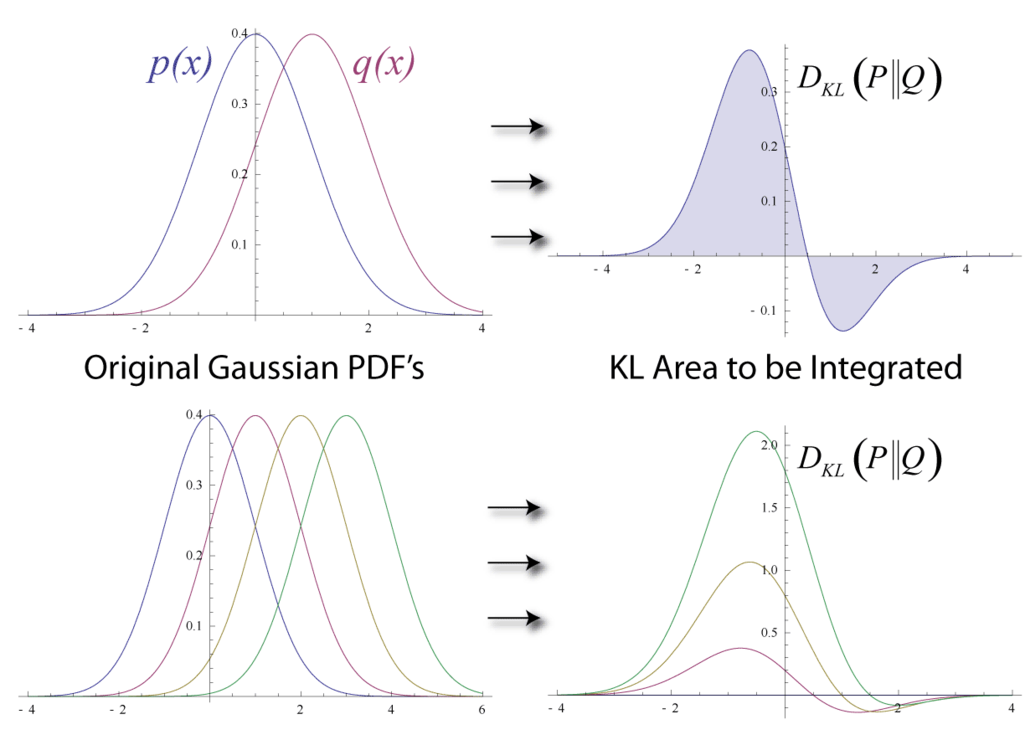
\includegraphics[height=0.8\textheight]{figs/kl.png}
            \caption{Taken from "Kullback–Leibler divergence", Wikipedia, CC BY-SA 3.0}
        \end{figure}
    \end{center}
\end{frame}

    \begin{frame}{Working through the math - 3}
        \begin{itemize}[<+->]
            \item Ignoring problems seemed like a good way to go :D
            \item Let's continue with that idea, parametrize a function Q and optimize it
        \end{itemize}
    \begin{align*}
        \onslide<+->{\mathcal{KL}[Q(z)||P(z|x)] =& \int Q(z) \log\left(\frac{Q(z)}{P(z|x)}\right)} \\\onslide<+->{&\mathbb{E}_{z\sim Q}[\log Q(z) - \log P(z|x)]}
    \end{align*}
        \begin{itemize}[<+->]
        \item Using Bayes rule:
    \end{itemize}
    \begin{align*}
        \onslide<+->{\mathcal{KL}[Q(z)||P(z|x)] = \mathbb{E}_{z\sim Q}[\log Q(z) - \log \frac{P(x|z) P(z)}{P(x)}]}\\
        \onslide<+->{= \mathbb{E}_{z\sim Q}[\log Q(z) - (\log P(x|z) + \log P(z) - \log P(x))]}\\
        \onslide<+->{= \mathbb{E}_{z\sim Q}[\log Q(z) - \log P(x|z) - \log P(z)] + \log P(x)}
    \end{align*}

\end{frame}

\begin{frame}{Working through the math - 4}
    \begin{align*}
        \onslide<+->{\mathcal{KL}[Q(z)||P(z|x)] = \mathbb{E}_{z\sim Q}[\log Q(z) - \log P(x|z) - \log P(z)] + \log P(x)}\\
        \onslide<+->{\log P(x) - \mathcal{KL}[Q(z)||P(z|x)] = \mathbb{E}_{z\sim Q}[\log P(x|z)] - \mathcal{KL}[Q(z)||P(z)]}
    \end{align*}

    \onslide<+->{What we have now:}
    \begin{itemize}[<+->]
        \item $\log P(x)$: maximization goal
        \item $\mathcal{KL}[Q(z)||P(z|x)]$: ``closeness'' of Q to P
        \item $\mathbb{E}_{z \sim Q}[\log P(x|z)]$: maximization of $P(x|z)$ with regards to Q
        \item $\mathcal{KL}[Q(z)||P(z)]$: regularization of Q on prior $P(z)$
    \end{itemize}

    \begin{itemize}[<+->]
        \item We can choose Q arbitrarily...
        \item ... so we can choose an entry which depends on x
    \end{itemize}

\end{frame}

\begin{frame}{Working through the math - 5}
    \begin{align*}
        \onslide<+->{\log P(x) - D[Q(z|x)||P(z|x)] = \mathbb{E}_{z\sim Q}[\log P(x|z)] - D[Q(z|x)||P(z)]}
    \end{align*}
    
    \begin{itemize}[<+->]
        \item Right hand side: ELBO (Evidence Lower BOund): maximization target
        \item $P(x|z)$ and $Q(z|x)$: decoder and encoder learned from the data
        \item $P(z)$: prior on latent variables
        \item $P(z|x)$ will hopefully be approximated well by $Q(z|x)$. (discussion later)
    \end{itemize}
\end{frame}
\begin{frame}{Working through the math - 6}
    \begin{itemize}[<+->]
        \item Can we optimize now?
        \item No, not yet: we still need to choose $Q(z|x)$ and work out some math
    \end{itemize}
    \begin{align*}
        \onslide<+->{Q(z|x) = \mathcal{N}(z|\mu(x;\theta),\Sigma(x;\theta))}
    \end{align*}

    \begin{itemize}[<+->]
        \item $Q(z|x)$ can now approximate arbitrary PDF via $\mu$
        \item $\Sigma$ represents noise
    \end{itemize}
\end{frame}

\begin{frame}{Final math slide!}
    \begin{itemize}[<+->]
        \item With choices, ($P(x|z)\sim\mathcal{N}$ and $Q(z|x)\sim\mathcal{N}$), KL has closed form solution
            \begin{itemize}
                \item possible for other PDFs too
            \end{itemize}
        \item KL depends on learnable functions $f$ and $\mu$
        \item We can use neural networks to approximate those!
        \item Are we finished now?
    \end{itemize}
\end{frame}

\section{Variational Autoencoders}

\begin{frame}{What is an autoencoder?}
	\begin{center}
            \begin{figure}
                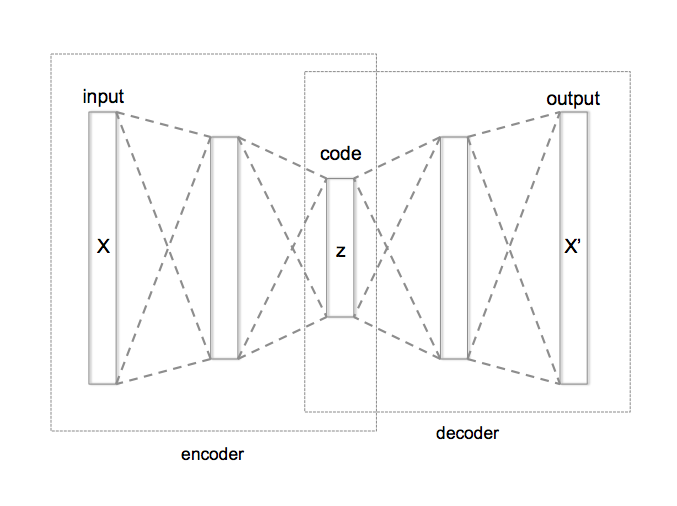
\includegraphics[height=.7\textheight]{figs/Autoencoder_structure.png}
                \caption{Taken from \url{https://commons.wikimedia.org/wiki/File:Autoencoder_structure.png}, (CC BY-SA 4.0)}
            \end{figure}
	\end{center}
\end{frame}

\begin{frame}{What is a variational autoencoder?}
	\begin{center}
            \begin{figure}
                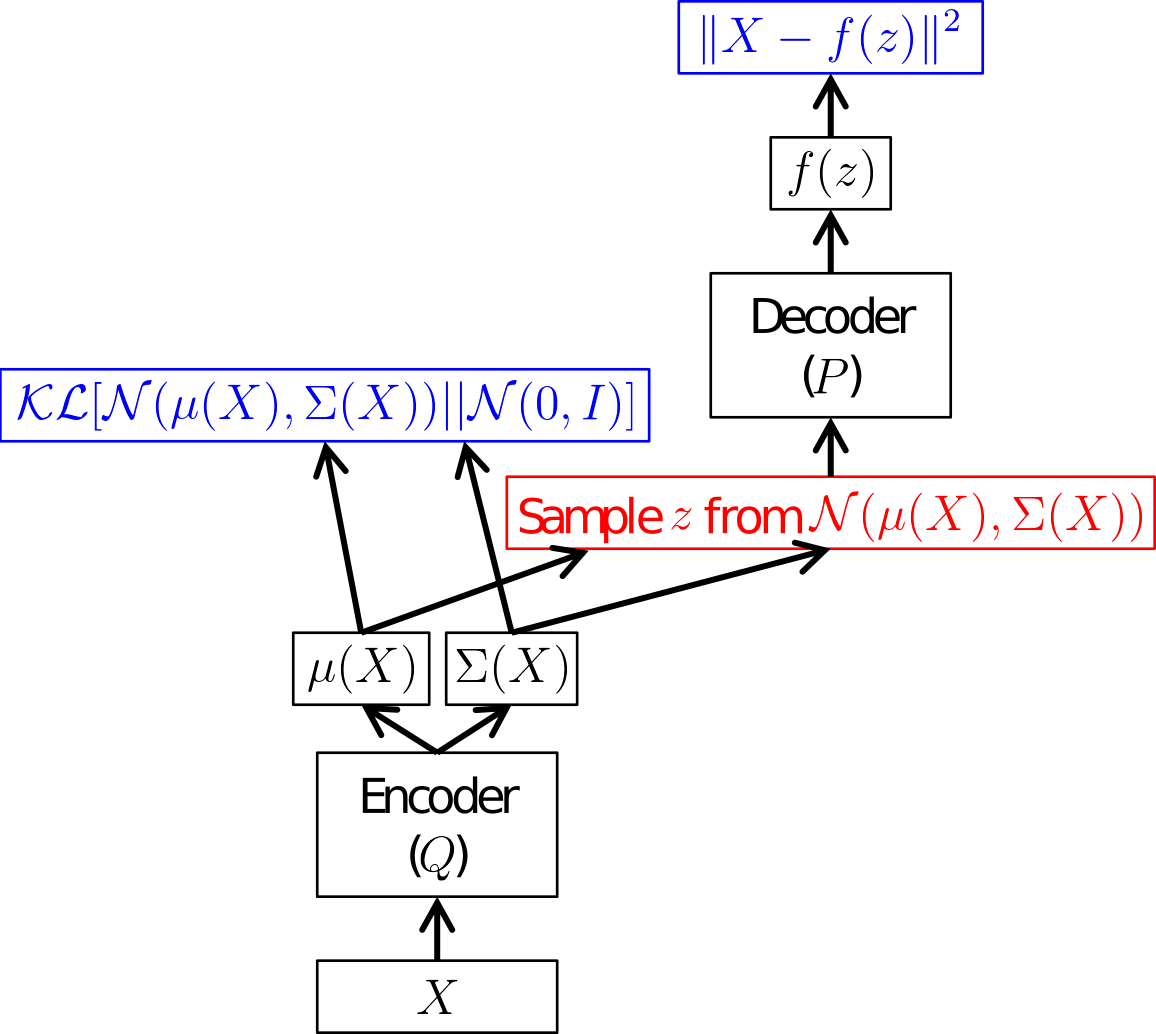
\includegraphics[height=.8\textheight]{figs/net.png}
                \caption{Taken from "Tutorial on Variational Autoencoders", Doersch, 2016}
            \end{figure}
	\end{center}
\end{frame}

\begin{frame}{Where is the trick?}
    \begin{minipage}[c]{0.3\textwidth}
            \begin{figure}
                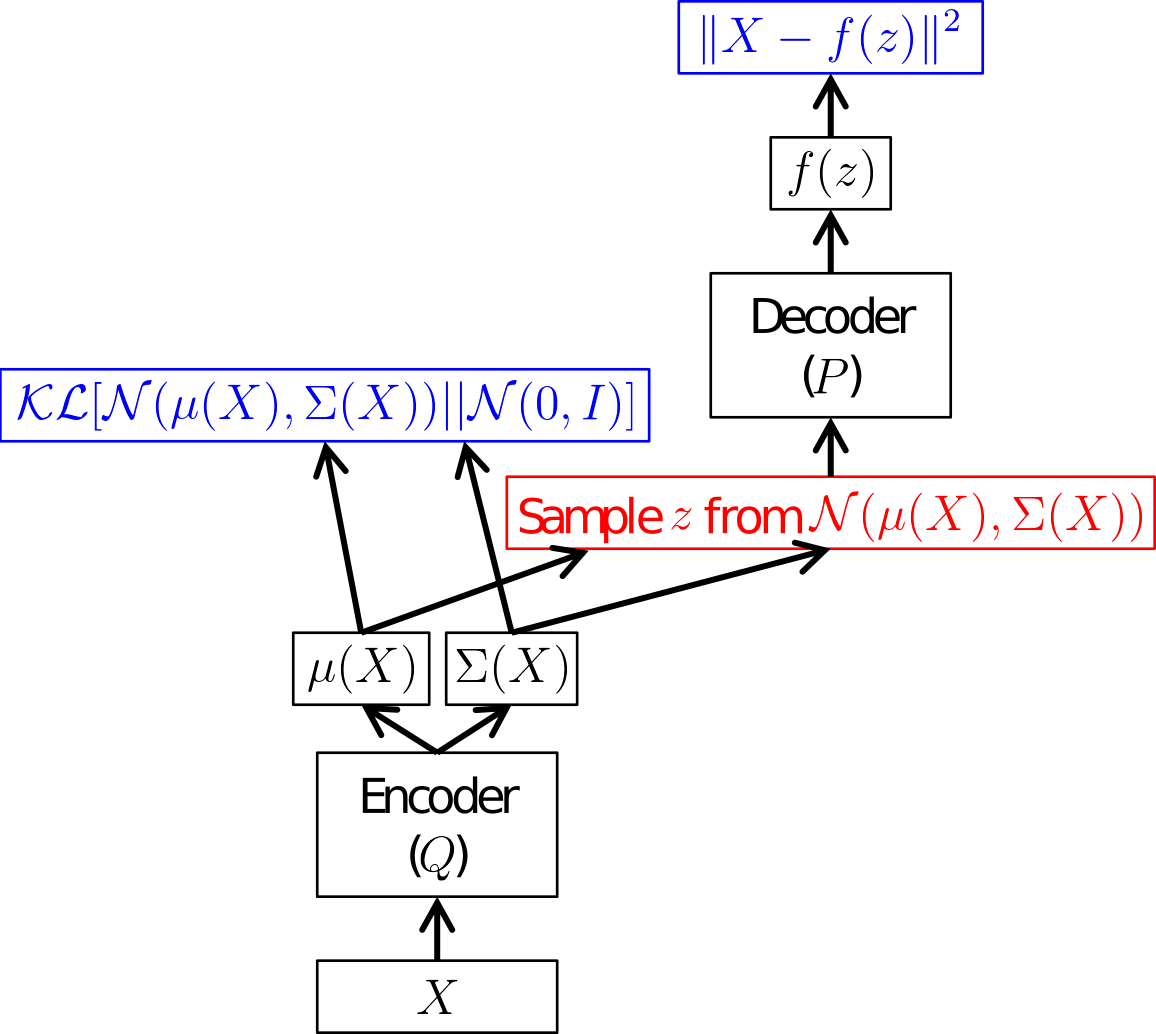
\includegraphics[width=.9\textwidth]{figs/net.png}
                %\caption{Taken from "Auto-Encoding Variational Bayes", Kingma \& Welling, 2014}
            \end{figure}
    \end{minipage}
    ~
    \begin{minipage}[c]{0.6\textwidth}
        \begin{itemize}[<+(1)->]
            \item ELBO is captured in the optimization by loss
            \item The problem is in backpropagation
            \item You can't propagate through a sampling layer
        \end{itemize}
    \end{minipage}
    
\end{frame}

\begin{frame}{All parts in detail}
	\begin{center}
            \begin{figure}
                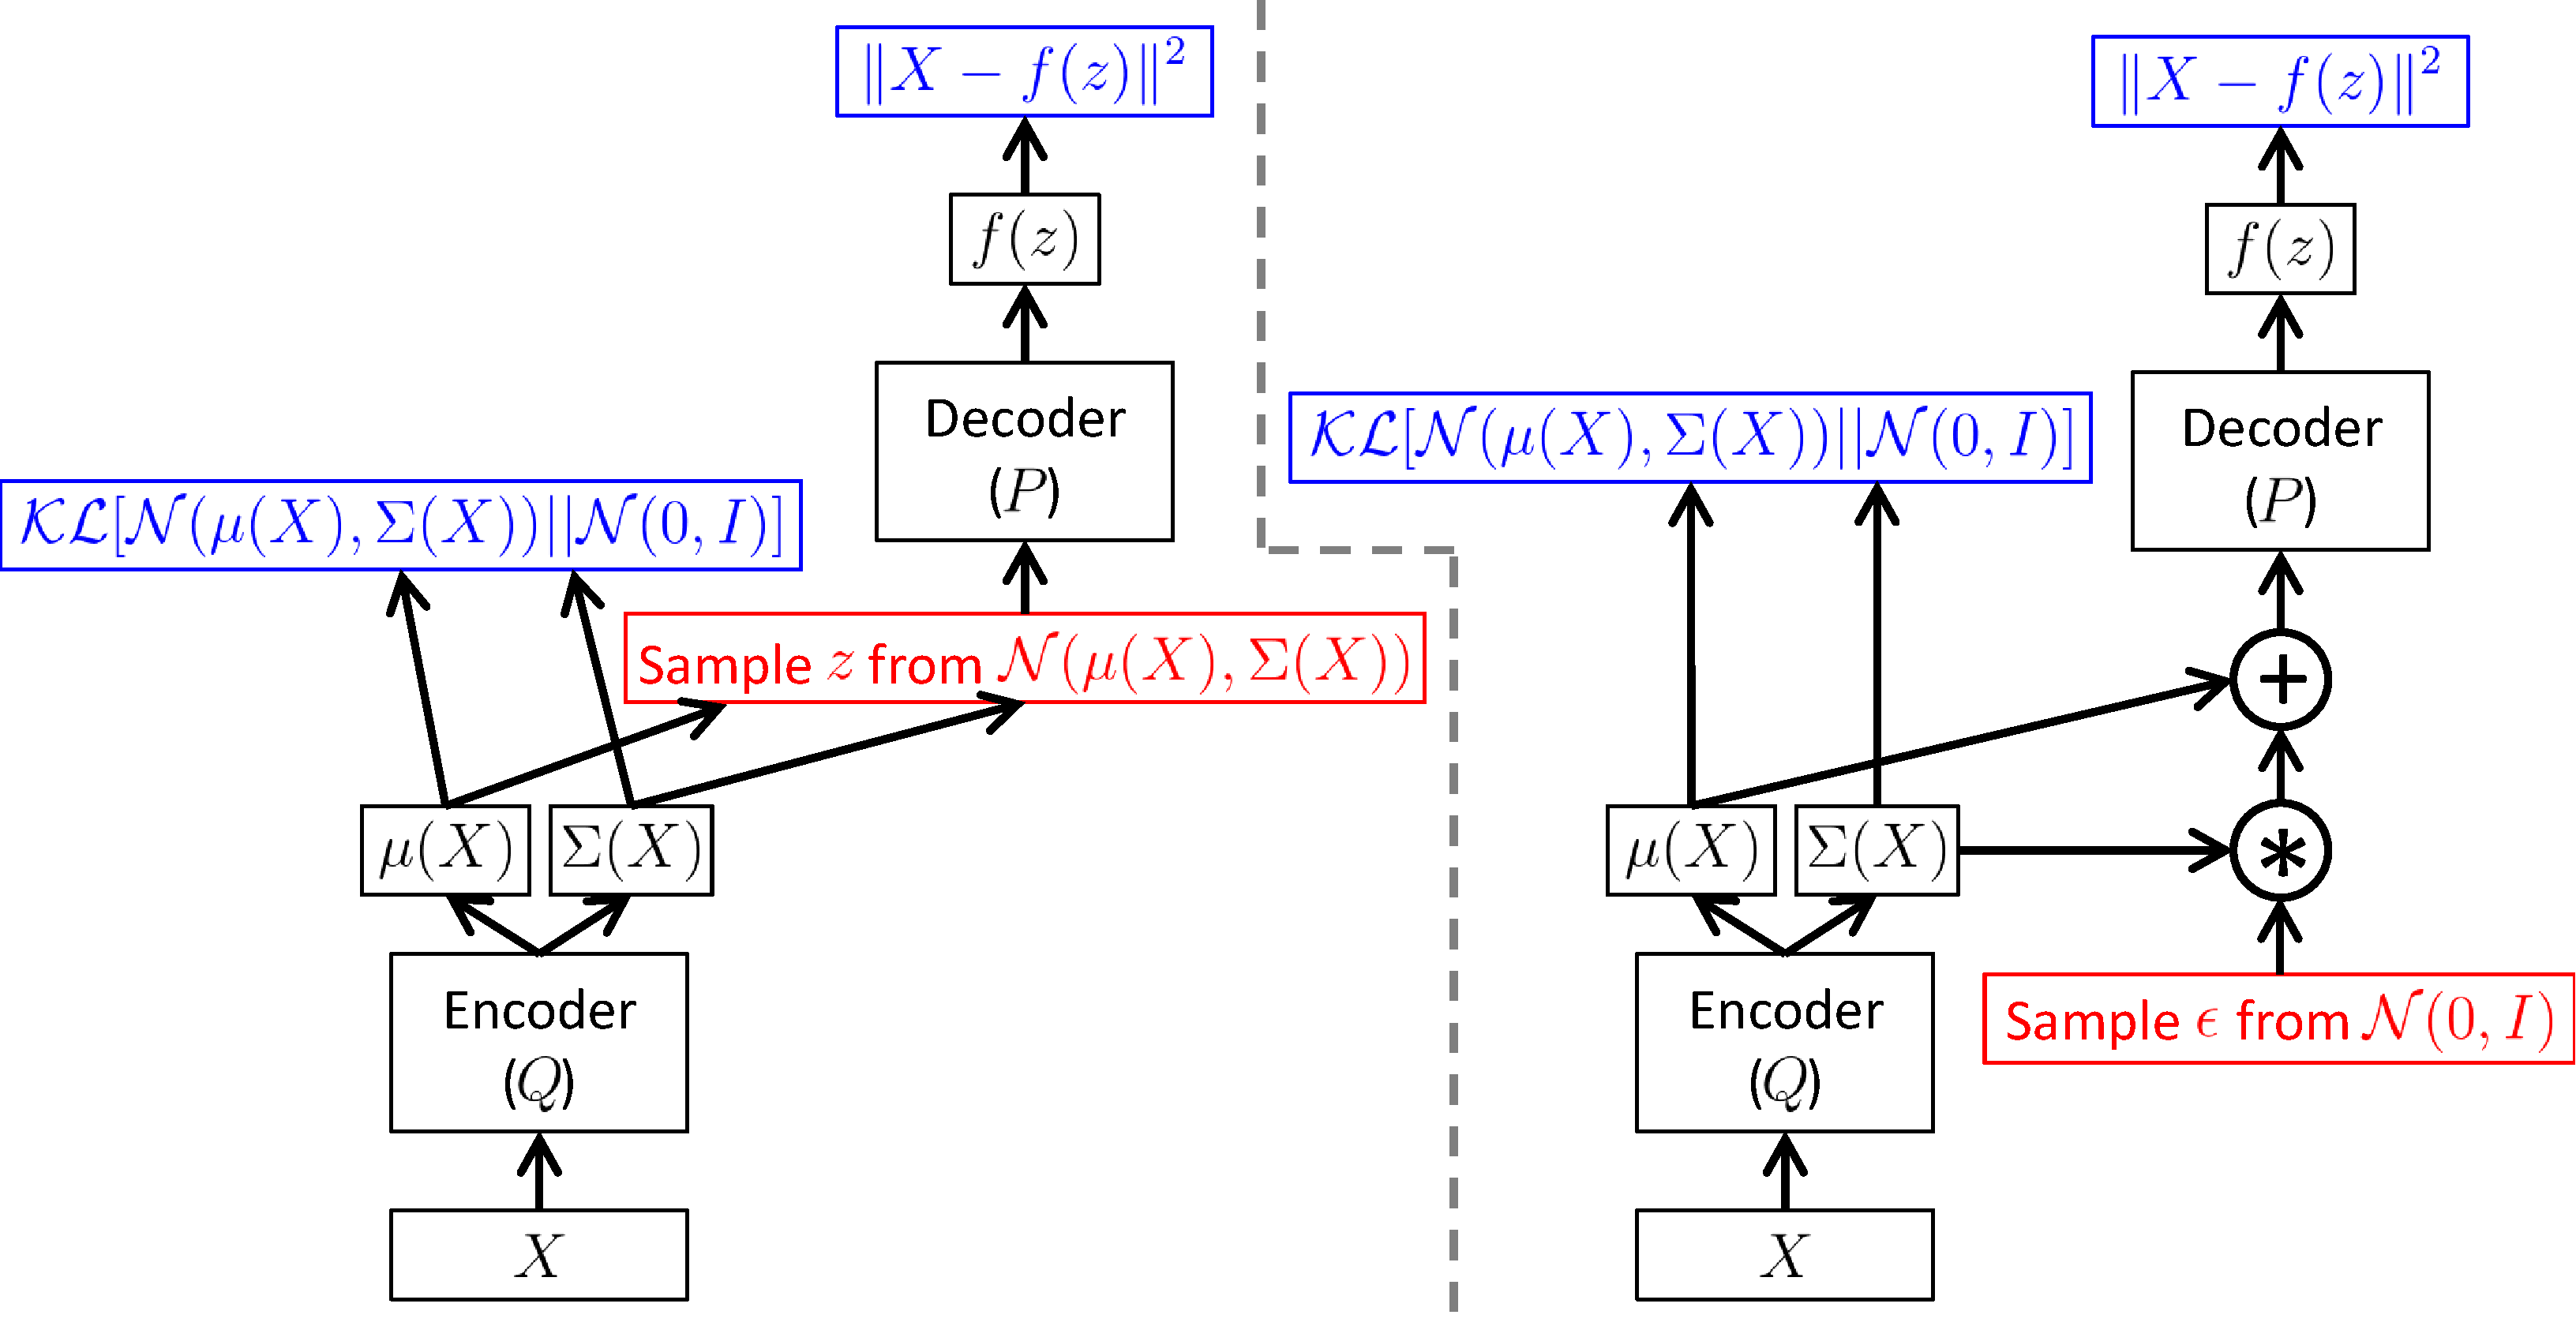
\includegraphics[width=.9\textwidth]{figs/net.pdf}
                \caption{Taken from "Tutorial on Variational Autoencoders", Doersch, 2016}
            \end{figure}
	\end{center}
\end{frame}

\begin{frame}{Why the sampling at all?}
    \begin{itemize}[<+->]
        \item We are trying to learn a distribution, not an encoder (per se)
        \item Encoder - decoder relations are deterministic
        \item How would we sample at inference time?
    \end{itemize}
    \begin{center}
    \onslide<+->{
        \begin{figure}
            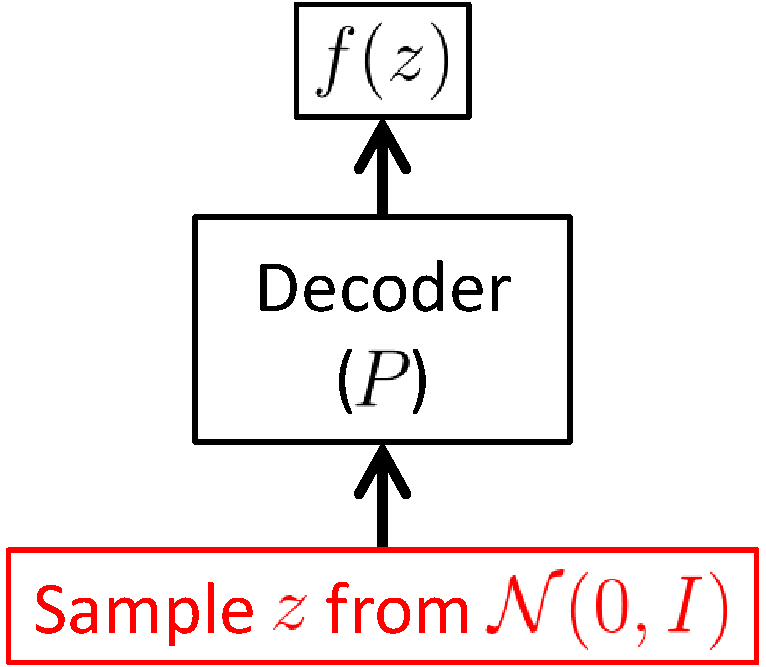
\includegraphics[height=0.4\textheight]{figs/test_time.pdf}
                \caption{Taken from "Tutorial on Variational Autoencoders", Doersch, 2016}
        \end{figure}}
    \end{center}
\end{frame}

\begin{frame}{Why use a variational autoencoder?}
    \begin{itemize}[<+->]
        \item Image generation is often done via GAN
        \item Is VAE obsolete?
    \end{itemize}
    \begin{table}
        \begin{tabularx}{\linewidth}{ l | X X }
            %\hline
            \onslide<+->{& VAE & GAN \\\hline\hline}
            \onslide<+->{Loss & L2 loss & adversarial loss}\\
            \onslide<+->{Latent & structured & unstructured}\\
            \onslide<+->{Results & blurry & sharp}\\
            \onslide<+->{Goal & generate good latent & generate good pictures}
            %\hline
        \end{tabularx}
    \end{table}
    \begin{itemize}[<+->]
        \item VAEs are density models, GAN not so much
        \item But the density is still intractable
        \item There is no mathematical guarantee for choosing a "good" latent
        \item L2 loss is computationally expensive, also does not capture ''visual closeness'' well
    \end{itemize}
\end{frame}


\section{Applications of VAE/VI}

\begin{frame}{VAE for generating images}
    \begin{figure}
        \begin{subfigure}[c]{0.4\textwidth}
            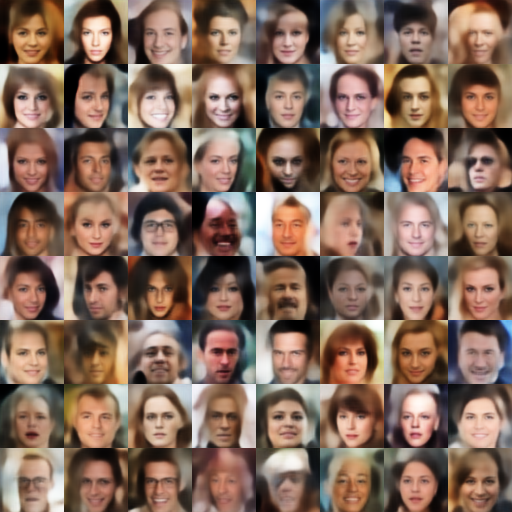
\includegraphics[width=\textwidth]{figs/vae_random.png}
                \caption{Taken from "Tutorial on Variational Autoencoders", Doersch, 2016}
        \end{subfigure}
        ~
        \begin{subfigure}[c]{0.4\textwidth}
            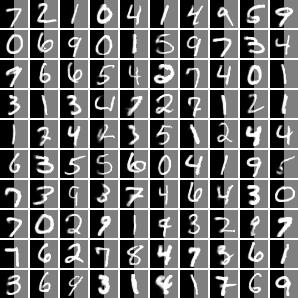
\includegraphics[width=\textwidth]{figs/cvae_out.png}
            \caption{Taken from GitHub \url{https://github.com/yzwxx/vae-celebA}}
        \end{subfigure}
    \end{figure}
\end{frame}

\begin{frame}{VAE for translations}
    \begin{figure}
        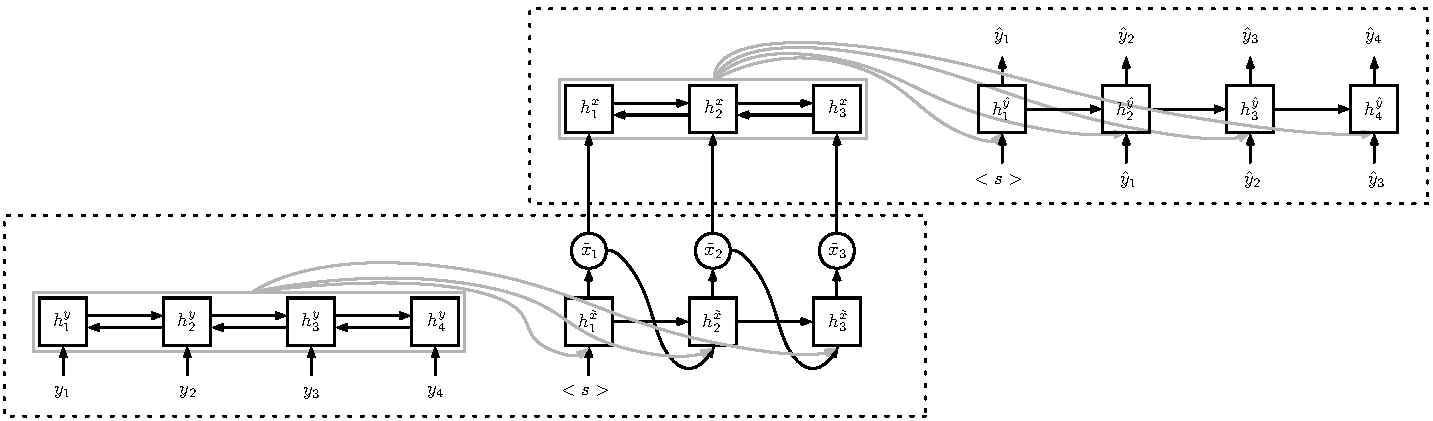
\includegraphics[width=\textwidth]{figs/Seq4model_overview.pdf}
        \caption{Taken from "Semantic Parsing with Semi-Supervised Sequential Autoencoders", Kocisky et al, 2016}
    \end{figure}
\end{frame}

\begin{frame}{More complex VAE usage}
    \begin{figure}
        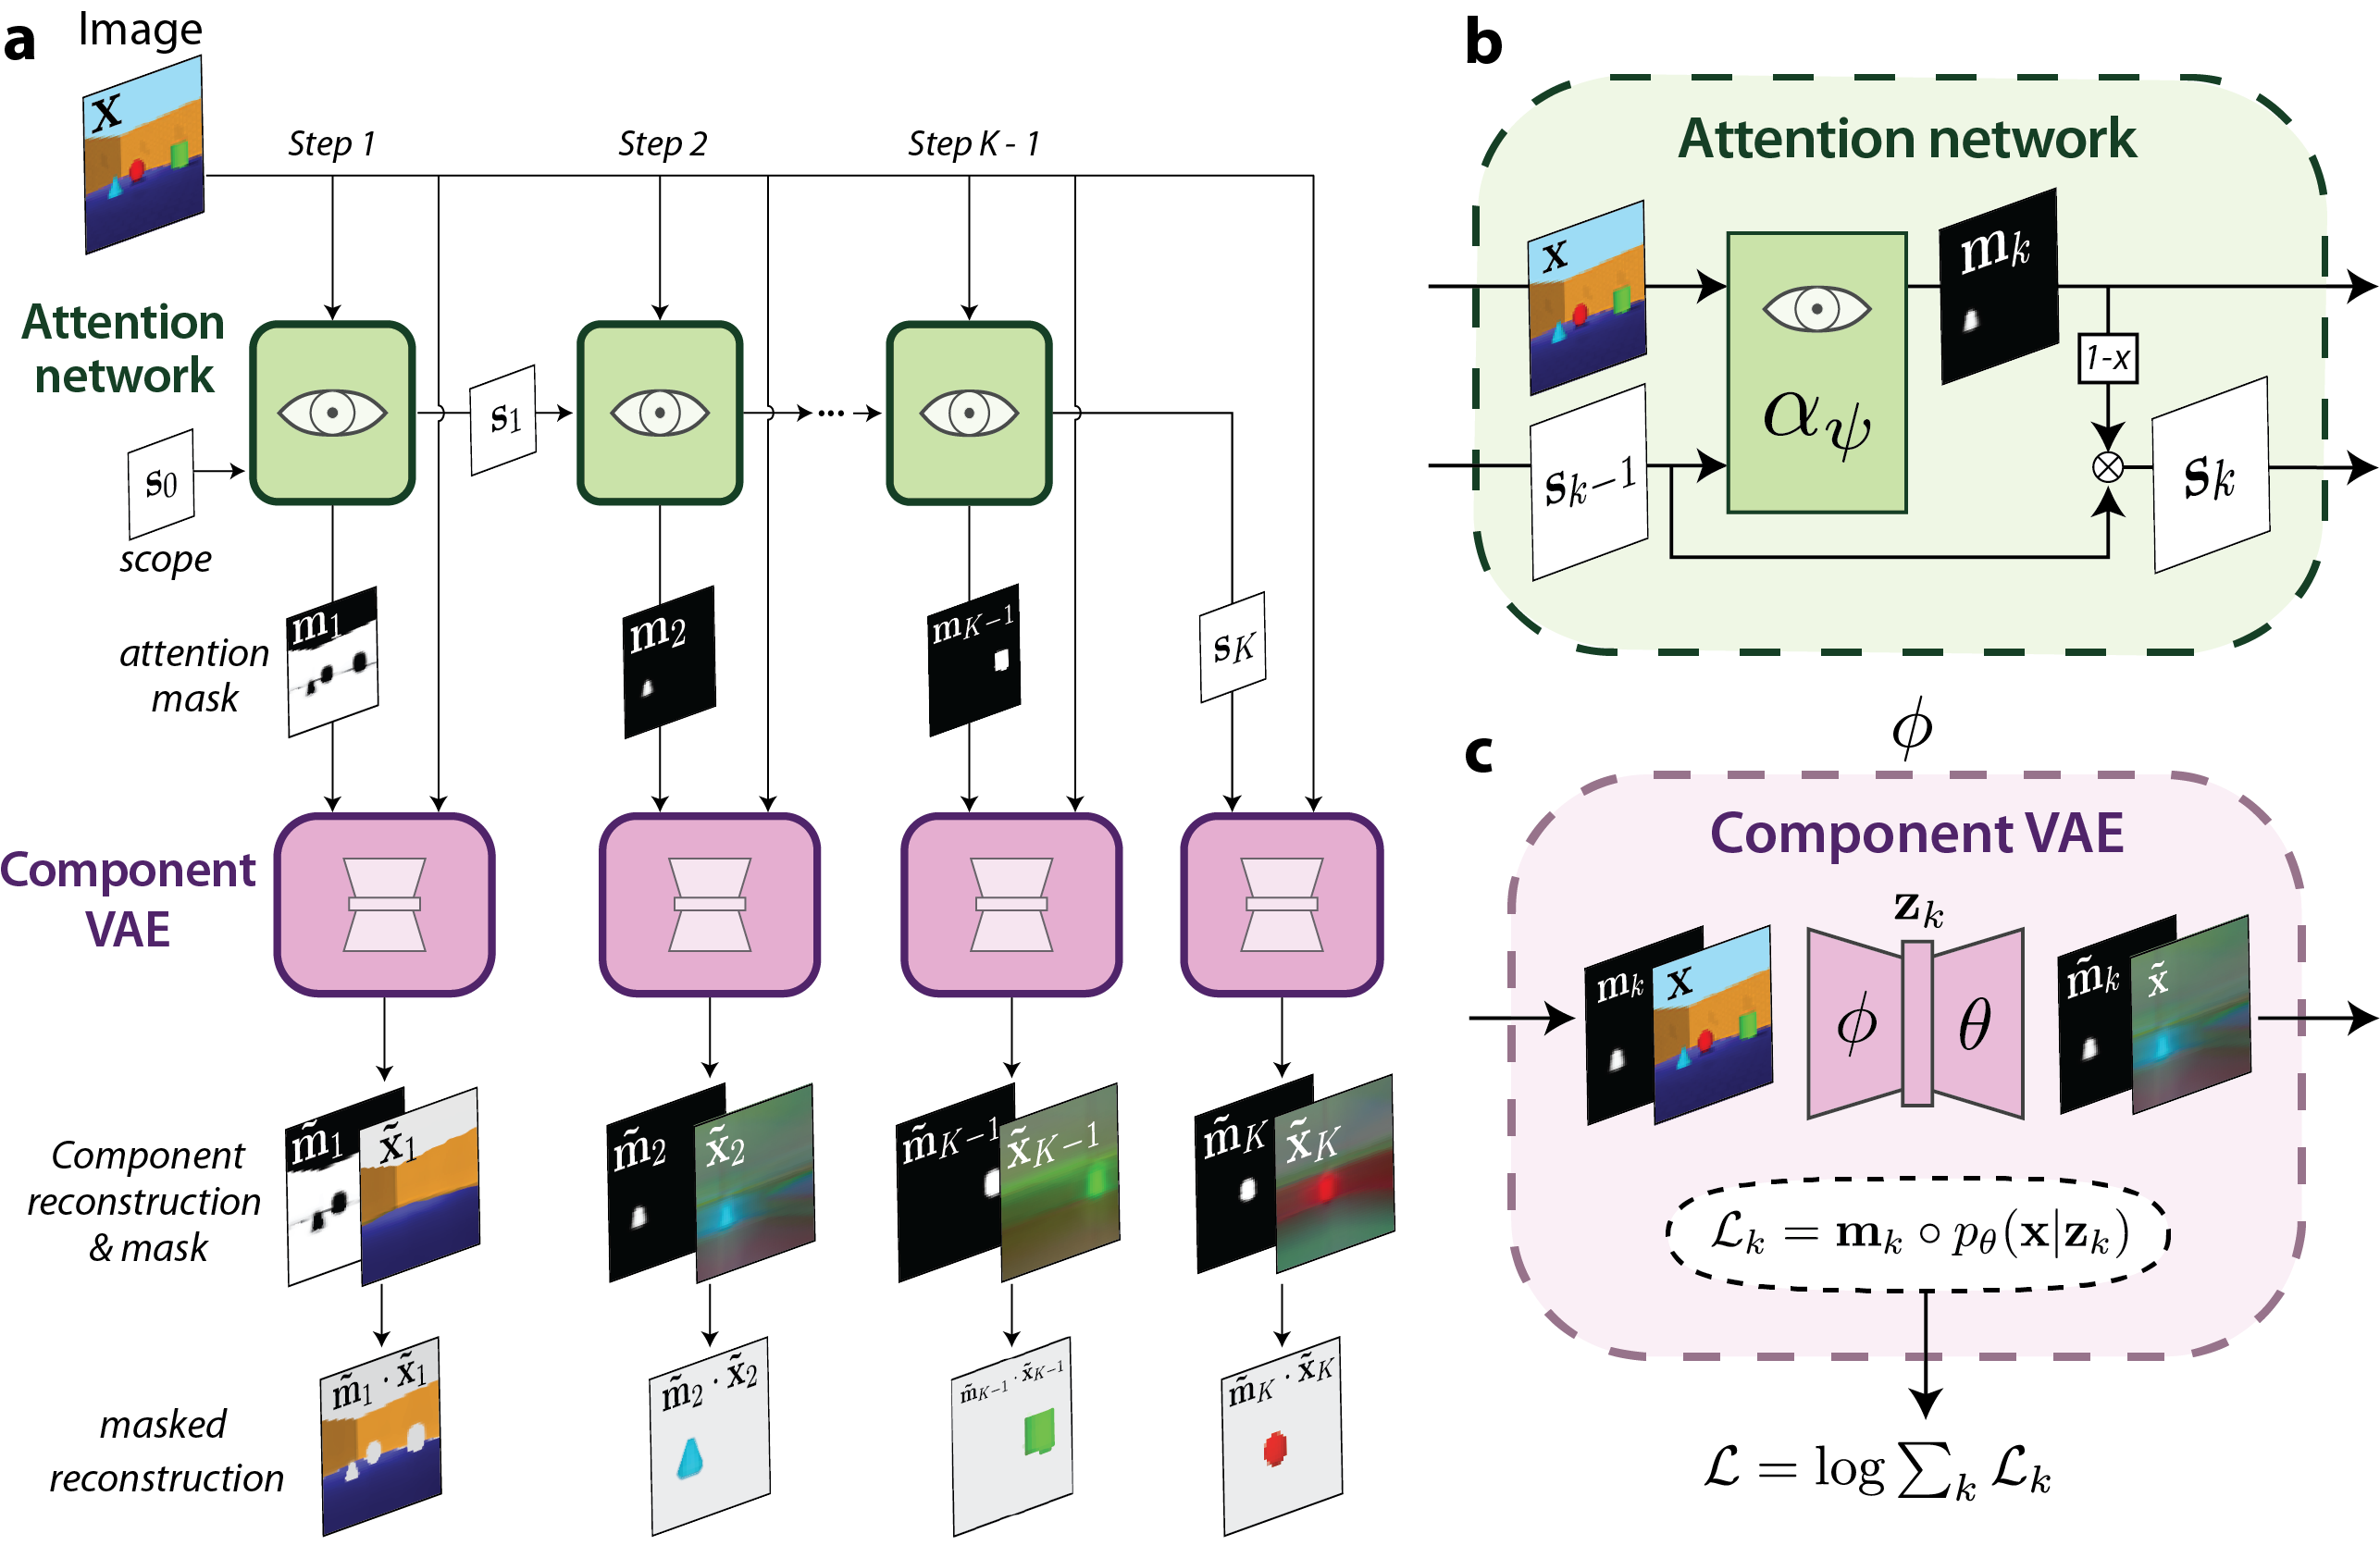
\includegraphics[height=0.7\textheight]{figs/monet_diagram_v2.png}
        \caption{Taken from "MONet: Unsupervised Scene Decomposition and Representation", Burgess et al., 2019}
    \end{figure}
\end{frame}

\begin{frame}{More complex VAE usage}
    \begin{figure}
        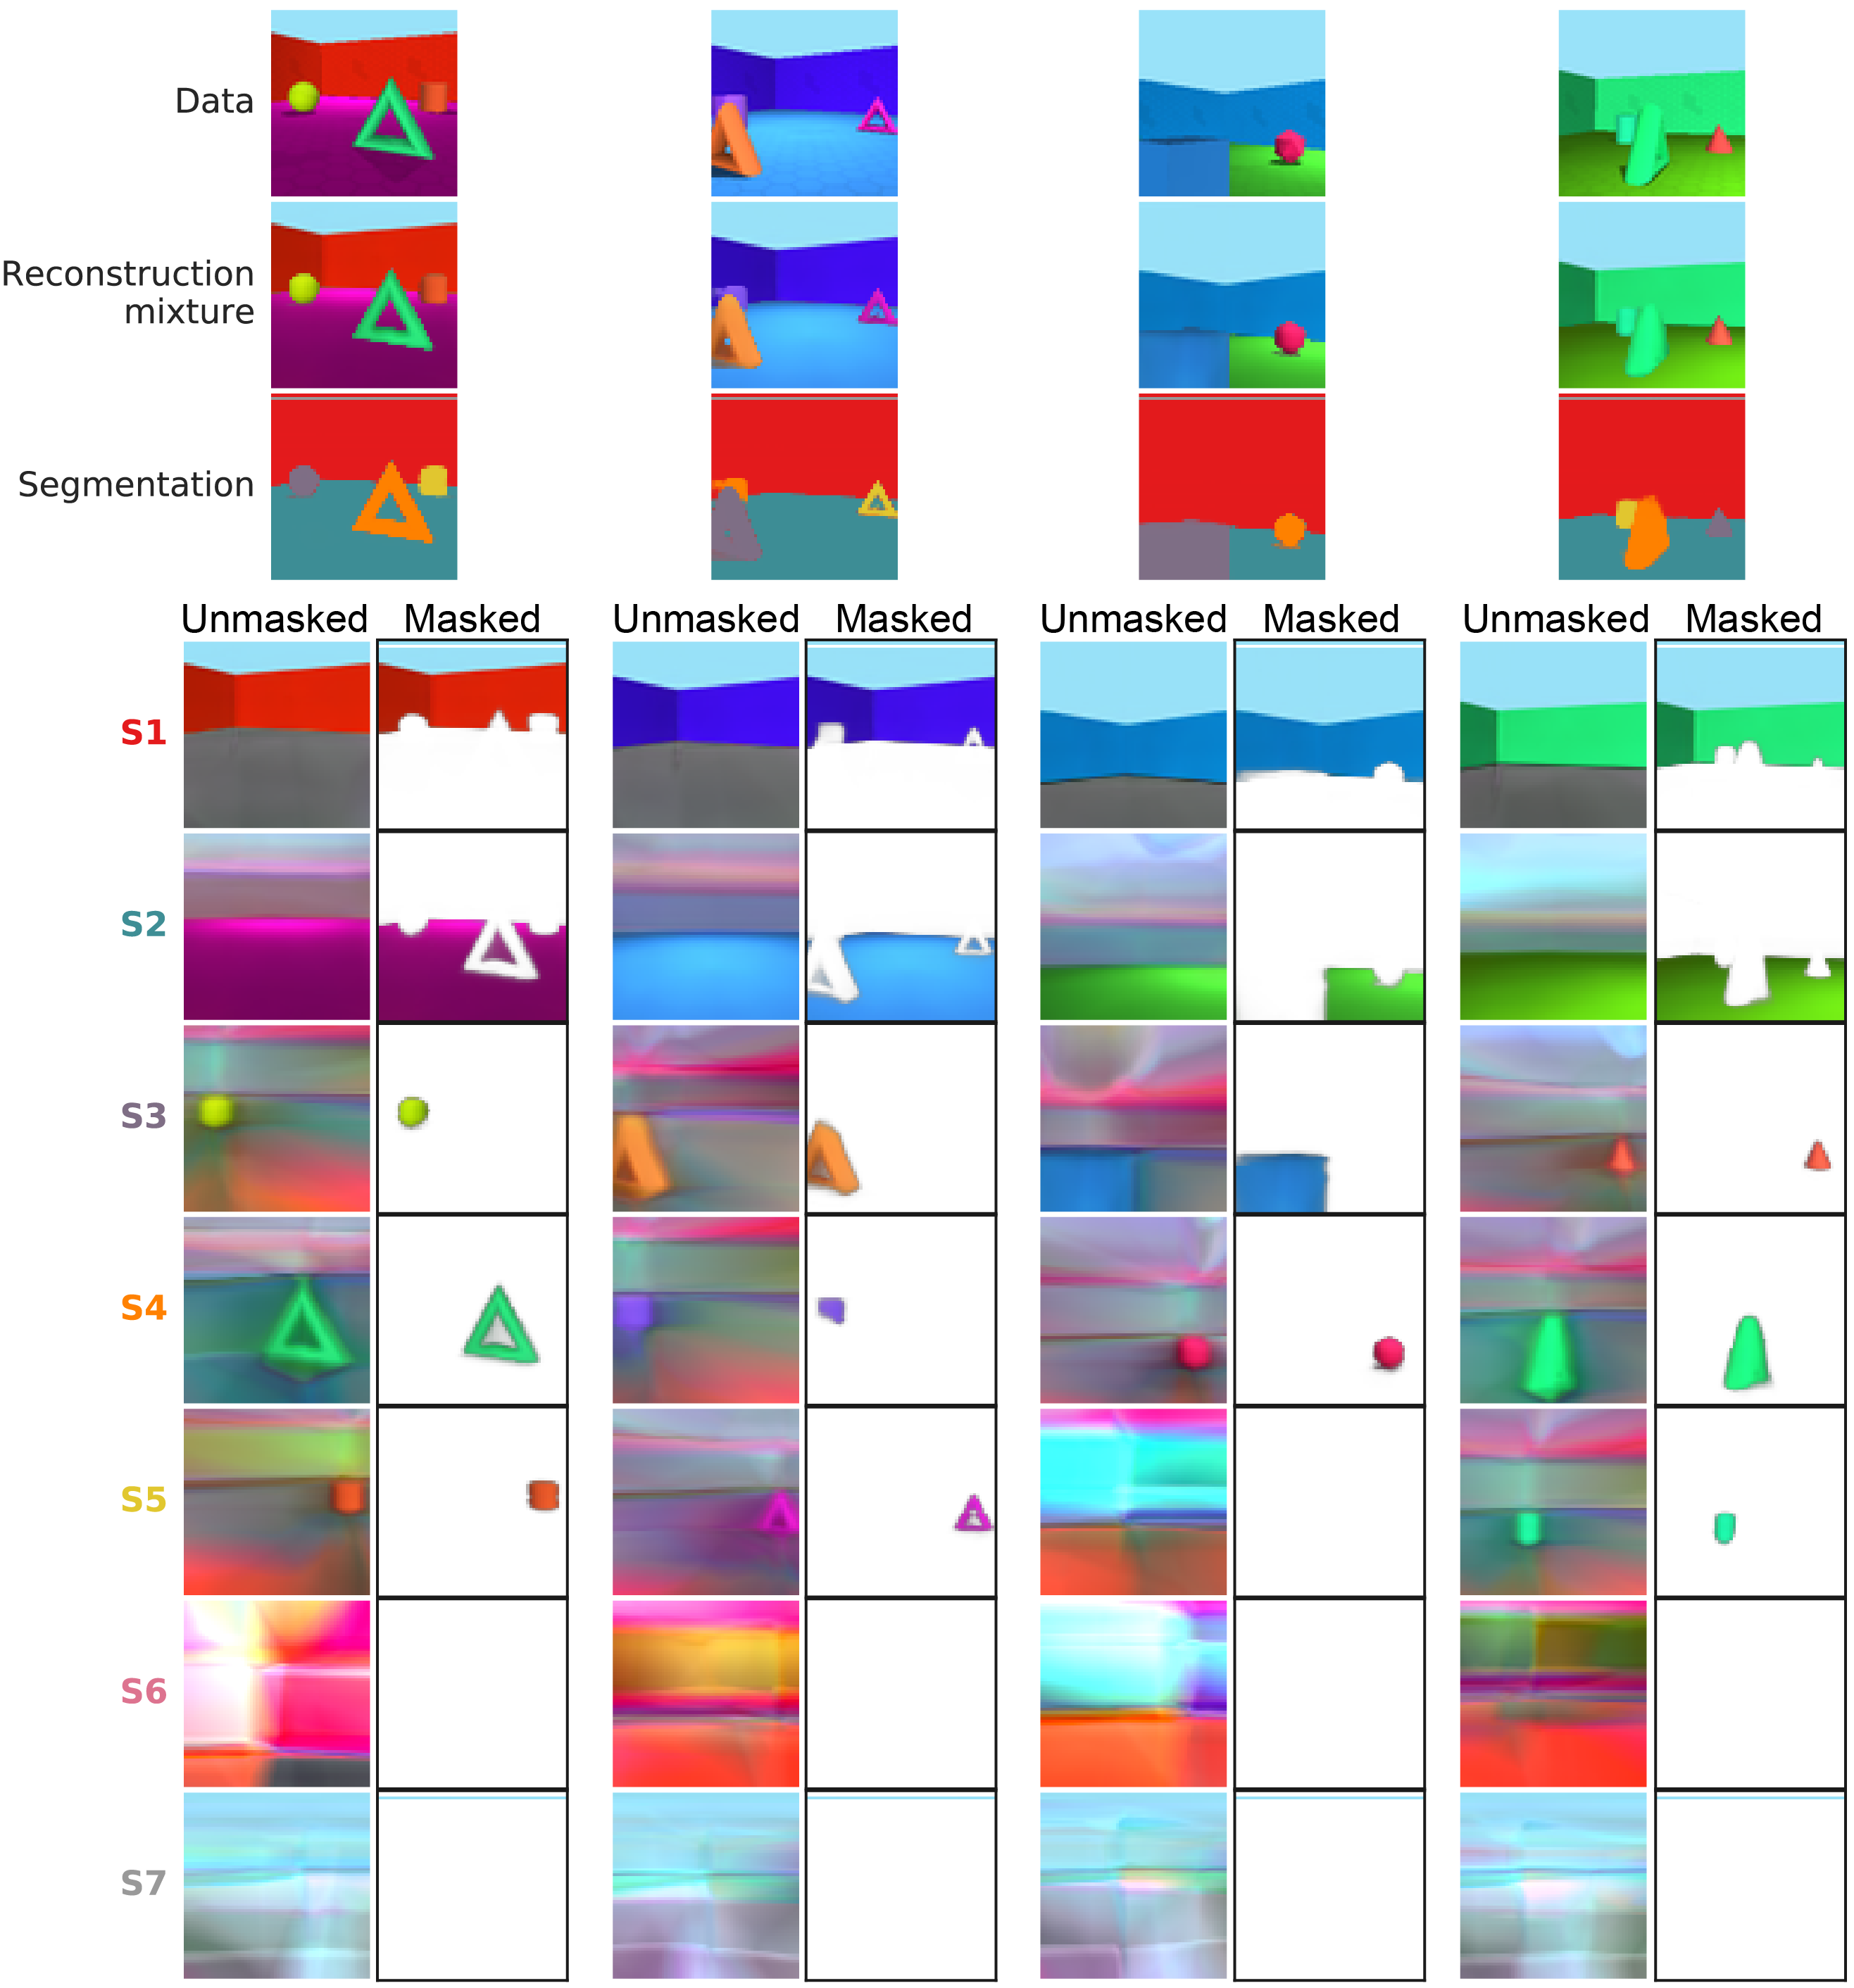
\includegraphics[height=0.7\textheight]{figs/monet_oir_decomposition_masked.png}
        \caption{Taken from "MONet: Unsupervised Scene Decomposition and Representation", Burgess et al., 2019}
    \end{figure}
\end{frame}

\begin{frame}{Learning a physics engine}
    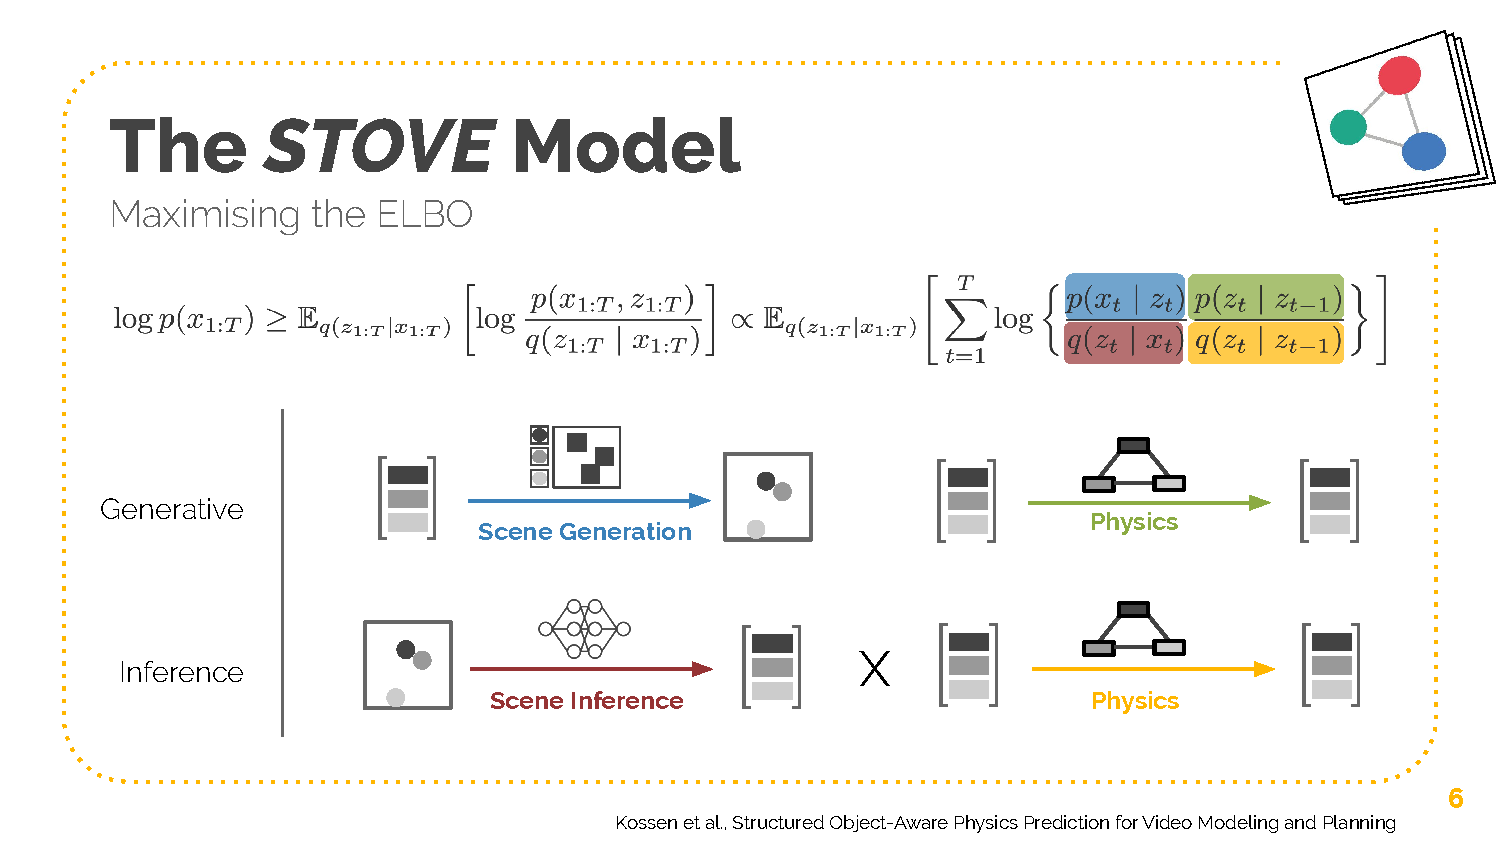
\includegraphics[width=\textwidth]{figs/stove-6.pdf}

\end{frame}

\begin{frame}{Further reading}
    \begin{itemize}
        \item "Stochastic Backpropagation and Approximate Inference in Deep Generative Models" by Danilo Rezende et al., 2014
        \item "Auto-Encoding Variational Bayes" by Durk Kingma and Max Welling, 2014
        \item "Tutorial on Variational Autoencoders" by Carl Doersch, 2016
        \item "Variational Inference: A Review for Statisticians" by David Blei et al., 2018
        \item "Improving Variational Inference with Inverse Autoregressive Flow" by Durk Kingma, 2016
        \item "Attend, Infer, Repeat: Fast Scene Understanding with Generative Models" by Ali Eslami et al., 2016
        \item "The Dreaming Variational Autoencoder for Reinforcement Learning Environments" by Per-Arne Andersen, 2018
    \end{itemize}
\end{frame}

\begin{frame}{Questions?}
    \center
    Any remaining questions?
\end{frame}

\appendix

\end{document}
